\chapter{Background}
\label{ch:background}

\section{Graphs and Laplacians}

Let $G = (V, E, w)$ be an undirected weighted graph with $n = |V|$ nodes and $m = |E|$ edges. Write $A \in \R^{n \times n}$ for its weighted adjacency matrix and $D = \diag(d_1, \dots, d_n)$ for the diagonal matrix of degrees $d_i = \sum_j A_{ij}$.

\begin{definition}[Graph Laplacian]
The \emph{combinatorial Laplacian} of $G$ is $L = D - A$. When no node is isolated, the \emph{normalized Laplacian} is
\begin{equation}
  \Lap = I - D^{-1/2} A D^{-1/2}.
  \label{eq:normalized-laplacian}
\end{equation}
\end{definition}

Both matrices are symmetric and positive semidefinite. For every $x \in \R^n$,
\begin{equation}
  x^\top L x = \frac{1}{2} \sum_{i,j} A_{ij} (x_i - x_j)^2,
  \label{eq:quadratic-form}
\end{equation}
so the quadratic form measures how much $x$ varies across edges.

\begin{proposition}
The eigenvalues of $\Lap$ lie in $[0, 2]$, and the multiplicity of the eigenvalue $0$ equals the number of connected components of $G$.
\end{proposition}

\section{Spectral embeddings}

Let $0 = \lambda_1 \le \lambda_2 \le \dots \le \lambda_n$ be the eigenvalues of $\Lap$ with orthonormal eigenvectors $u_1, \dots, u_n$. The \emph{spectral embedding} of dimension $k$ maps node $i$ to the $i$-th row of $U_k = [u_1, \dots, u_k]$. By the Courant--Fischer theorem, $U_k$ solves
\[
  \min_{X \in \R^{n \times k}} \tr\left( X^\top \Lap X \right) \quad \text{subject to} \quad X^\top X = I_k .
\]

\section{Graph filters}

A \emph{spectral filter} is a function $g \colon [0, 2] \to \R$ applied to the Laplacian through its eigendecomposition, $g(\Lap) = U g(\Lambda) U^\top$. Graph convolutional networks~\cite{kipf2017semi} use the linear filter $g(\lambda) = 1 - \lambda$; Chebyshev networks~\cite{defferrard2016convolutional} use polynomials of higher degree.

\begin{figure}[ht]
  \centering
  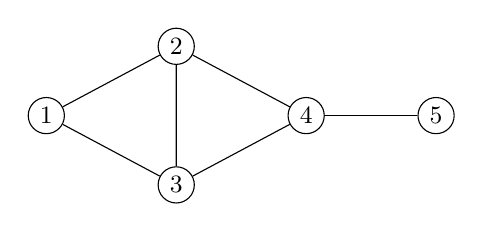
\begin{tikzpicture}[scale=1.1, every node/.style={circle, draw, inner sep=2pt, font=\small}]
    \node (a) at (0,0) {1};
    \node (b) at (1.5,0.8) {2};
    \node (c) at (1.5,-0.8) {3};
    \node (d) at (3,0) {4};
    \node (e) at (4.5,0) {5};
    \draw (a) -- (b) -- (d) -- (c) -- (a);
    \draw (b) -- (c);
    \draw (d) -- (e);
  \end{tikzpicture}
  \caption{A graph with five nodes. Removing the edge between nodes 4 and 5 disconnects it, which the second eigenvalue of the Laplacian detects.}
  \label{fig:example-graph}
\end{figure}
